\newpage
\section{Tiered Compilation Thresholds}
\label{a:compilethresholds}
\begin{table}[h]
  \centering
 % \caption{}
  \label{t:compilethresholds}
  \begin{center}
    \begin{tabular}{| l | p{9.0cm} | r | }
       \hline
       \textbf{flag} & \textbf{description} & \textbf{default} \\ \hline\hline
       CompileThresholdScaling & number of interpreted method invocations before (re-)compiling & 1.0\\ \hline
       Tier0InvokeNotifyFreqLog & Interpreter (tier 0) invocation notification frequency & 7\\ \hline
       Tier2InvokeNotifyFreqLog & C1 without MDO (tier 2) invocation notification frequency & 11 \\ \hline
       Tier3InvokeNotifyFreqLog & C1 with MDO profiling (tier 3) invocation notification frequency & 10 \\ \hline
       Tier23InlineeNotifyFreqLog & Inlinee invocation (tiers 2 and 3) notification frequency & 20 \\ \hline
       Tier0BackedgeNotifyFreqLog & Interpreter (tier 0) invocation notification frequency & 10 \\ \hline
       Tier2BackedgeNotifyFreqLog & C1 without MDO (tier 2) invocation notification frequency & 14 \\ \hline
       Tier3BackedgeNotifyFreqLog & C1 with MDO profiling (tier 3) invocation notification frequency & 13 \\ \hline
       Tier2CompileThreshold & threshold at which tier 2 compilation is invoked & 0 \\ \hline
       Tier2BackEdgeThreshold & Back edge threshold at which tier 2 compilation is invoked & 0 \\ \hline
       Tier3InvocationThreshold & Compile if number of method invocations crosses this threshold & 200 \\ \hline
       Tier3MinInvocationThreshold & Minimum invocation to compile at tier 3 & 100 \\ \hline
       Tier3CompileThreshold & Threshold at which tier 3 compilation is invoked (invocation minimum must be satisfied) & 2000 \\ \hline
       Tier3BackEdgeThreshold & Back edge threshold at which tier 3 OSR compilation is invoked & 60000 \\ \hline
       Tier4InvocationThreshold & Compile if number of method invocations crosses this threshold & 5000 \\ \hline
       Tier4MinInvocationThreshold & Minimum invocation to compile at tier 4 & 600 \\ \hline
       Tier4CompileThreshold & Threshold at which tier 4 compilation is invoked (invocation minimum must be satisfied) & 15000 \\ \hline
       Tier4BackEdgeThreshold & Back edge threshold at which tier 4 OSR compilation is invoked & 40000 \\ \hline
    \end{tabular}
  \end{center}
\end{table}
\newpage
\section{Cached Profile Example}
\label{a:cacheprofileexample}
\begin{lstlisting}[caption=Example of cached profiling information,label=l:cacheprofileexample,language=Java]
# 189 ciObject found
ciMethod java/lang/Double toString (D)Ljava/lang/String; 25 1 7 0 0
ciMethod java/lang/Long toString (J)Ljava/lang/String; 9 1 3 0 0
ciMethod java/lang/Long valueOf (J)Ljava/lang/Long; 25 1 7 0 0
ciMethod java/lang/Long longValue ()J 9 1 3 0 -1
ciMethodData java/lang/Double toString (D)Ljava/lang/String; 1 7 orig 280 152 101 83 95 3 127 0 0 88 140 138 72 3 127 0 0 144 1 0 0 0 0 0 0 0 0 0 0 0 0 0 0 0 0 0 0 0 0 0 0 0 0 0 0 0 0 0 0 0 0 0 0 0 0 0 0 0 0 0 0 0 0 0 0 0 0 0 0 0 0 0 0 0 0 0 0 0 0 0 0 77 68 79 32 101 120 116 114 97 32 100 97 116 97 32 108 111 99 107 0 0 0 0 0 0 0 0 0 0 0 0 0 0 0 0 0 0 0 0 0 0 0 0 0 0 0 0 0 0 0 0 0 0 0 0 0 0 0 0 0 0 0 0 0 0 0 0 0 0 0 0 0 0 0 0 0 0 0 0 0 0 0 0 0 0 0 0 0 0 0 0 0 0 0 0 0 0 0 0 0 0 0 0 0 0 0 0 0 0 0 0 0 0 0 0 0 0 0 0 0 0 0 0 0 0 0 0 0 0 0 0 0 0 0 0 0 3 0 0 0 33 0 0 0 1 0 0 0 0 0 0 0 0 0 0 0 0 0 0 0 248 3 0 0 248 31 0 0 2 0 0 0 0 0 0 0 0 0 0 0 48 0 0 0 254 255 255 255 0 0 0 0 2 0 4 0 0 0 0 0 data 16 0x40002 0x4 0x80002 0x4 0xf0002 0x4 0x0 0x0 0x0 0x0 0x0 0x0 0x9 0x2 0x0 0x0 oops 0 methods 0
ciMethodData java/lang/Long toString (J)Ljava/lang/String; 1 3 orig 280 152 101 83 95 3 127 0 0 248 47 139 72 3 127 0 0 40 2 0 0 136 0 0 0 0 0 0 0 0 0 0 0 0 0 0 0 0 0 0 0 0 0 0 0 0 0 0 0 0 0 0 0 0 0 0 0 0 0 0 0 0 0 0 0 0 0 0 0 0 0 0 0 0 0 0 0 0 0 0 0 77 68 79 32 101 120 116 114 97 32 100 97 116 97 32 108 111 99 107 0 0 0 0 0 0 0 0 0 0 0 0 0 0 0 0 0 0 0 0 0 0 0 0 0 0 0 0 0 0 0 0 0 0 0 0 0 0 0 0 0 0 0 0 0 0 0 0 0 0 0 0 0 0 0 0 0 0 0 0 0 0 0 0 0 0 0 0 0 0 0 0 0 0 0 0 0 0 0 0 0 0 0 0 0 0 0 0 0 0 0 0 0 0 0 0 0 0 0 0 0 0 0 0 0 0 0 0 0 0 0 0 0 0 0 0 0 1 0 0 0 17 0 0 0 1 0 0 0 0 0 0 0 0 0 0 0 0 0 0 0 248 3 0 0 248 31 0 0 2 0 0 0 0 0 0 0 0 0 0 0 200 0 0 0 254 255 255 255 0 0 0 0 2 0 5 0 0 0 0 0 data 35 0x50002 0x2 0xd0007 0x2 0x30 0x0 0x170002 0x0 0x1e0007 0x2 0x48 0x0 0x230002 0x0 0x280003 0x0 0x28 0x2c0002 0x2 0x370002 0x2 0x400002 0x2 0x480002 0x2 0x0 0x0 0x0 0x0 0x0 0x0 0x9 0x2 0x0 0x0 oops 0 methods 0
ciMethodData java/lang/Long valueOf (J)Ljava/lang/Long; 1 7 orig 280 152 101 83 95 3 127 0 0 232 61 139 72 3 127 0 0 224 1 0 0 80 0 0 0 0 0 0 0 0 0 0 0 0 0 0 0 0 0 0 0 0 0 0 0 0 0 0 0 0 0 0 0 0 0 0 0 0 0 0 0 0 0 0 0 0 0 0 0 0 0 0 0 0 0 0 0 0 0 0 0 77 68 79 32 101 120 116 114 97 32 100 97 116 97 32 108 111 99 107 0 0 0 0 0 0 0 0 0 0 0 0 0 0 0 0 0 0 0 0 0 0 0 0 0 0 0 0 0 0 0 0 0 0 0 0 0 0 0 0 0 0 0 0 0 0 0 0 0 0 0 0 0 0 0 0 0 0 0 0 0 0 0 0 0 0 0 0 0 0 0 0 0 0 0 0 0 0 0 0 0 0 0 0 0 0 0 0 0 0 0 0 0 0 0 0 0 0 0 0 0 0 0 0 0 0 0 0 0 0 0 0 0 0 0 0 0 3 0 0 0 33 0 0 0 1 0 0 0 0 0 0 0 0 0 0 0 0 0 0 0 248 3 0 0 248 31 0 0 2 0 0 0 0 0 0 0 0 0 0 0 128 0 0 0 254 255 255 255 0 0 0 0 2 0 5 0 0 0 0 0 data 26 0x50002 0x4 0xd0007 0x0 0x50 0x4 0x150007 0x4 0x30 0x0 0x270002 0x0 0x300002 0x4 0x380002 0x4 0x0 0x0 0x0 0x0 0x0 0x0 0x9 0x2 0x0 0x0 oops 0 methods 0
ciMethodData java/lang/Long longValue ()J 1 3 orig 280 152 101 83 95 3 127 0 0 176 67 139 72 3 127 0 0 120 1 0 0 0 0 0 0 0 0 0 0 0 0 0 0 0 0 0 0 0 0 0 0 0 0 0 0 0 0 0 0 0 0 0 0 0 0 0 0 0 0 0 0 0 0 0 0 0 0 0 0 0 0 0 0 0 0 0 0 0 0 0 0 77 68 79 32 101 120 116 114 97 32 100 97 116 97 32 108 111 99 107 0 0 0 0 0 0 0 0 0 0 0 0 0 0 0 0 0 0 0 0 0 0 0 0 0 0 0 0 0 0 0 0 0 0 0 0 0 0 0 0 0 0 0 0 0 0 0 0 0 0 0 0 0 0 0 0 0 0 0 0 0 0 0 0 0 0 0 0 0 0 0 0 0 0 0 0 0 0 0 0 0 0 0 0 0 0 0 0 0 0 0 0 0 0 0 0 0 0 0 0 0 0 0 0 0 0 0 0 0 0 0 0 0 0 0 0 0 1 0 0 0 17 0 0 0 1 0 0 0 0 0 0 0 0 0 0 0 0 0 0 0 248 3 0 0 248 31 0 0 2 0 0 0 0 0 0 0 0 0 0 0 32 0 0 0 254 255 255 255 0 0 0 0 2 0 5 0 0 0 0 0 data 13 0x50002 0x2 0x110002 0x2 0x0 0x0 0x0 0x0 0x0 0x0 0x9 0x1 0x0 oops 0 methods 0
ciMethod NoCompile method1 (D)D 17 80000001 4 0 -1
ciMethodData NoCompile method1 (D)D 2 30002544 orig 280 152 101 83 95 3 127 0 0 200 8 192 72 3 127 0 0 40 5 0 0 112 1 0 0 0 0 0 0 0 0 0 0 0 0 0 0 0 0 0 0 0 0 0 0 0 0 0 0 0 0 0 0 0 0 0 0 0 0 0 0 0 0 0 0 0 0 0 0 0 0 0 0 0 0 0 0 0 0 0 0 77 68 79 32 101 120 116 114 97 32 100 97 116 97 32 108 111 99 107 0 0 0 0 0 0 0 0 0 0 0 0 0 0 0 0 0 0 0 0 0 0 0 0 0 0 0 0 0 0 0 0 0 0 0 0 0 0 0 0 0 0 0 0 0 0 0 0 0 0 0 0 0 0 0 0 0 0 0 0 0 0 0 0 0 0 0 0 0 0 0 0 0 0 0 0 0 0 0 0 0 0 0 0 0 0 0 0 0 0 0 0 0 0 0 0 0 0 0 0 0 0 0 0 0 0 0 0 0 0 0 0 0 0 0 0 0 128 150 152 0 17 0 0 0 193 170 137 9 0 0 0 0 0 0 0 0 0 0 0 0 0 0 0 0 56 0 0 0 2 0 0 0 1 0 12 0 2 0 0 0 200 3 0 0 254 255 255 255 0 0 0 0 2 0 4 0 0 0 0 0 data 131 0x40002 0x2 0xa0007 0x0 0x130 0x2 0x140002 0x2 0x190005 0x0 0x7f03580bbc90 0x2 0x0 0x0 0x1d0002 0x2 0x200005 0x0 0x7f03580bbc90 0x2 0x0 0x0 0x250005 0x0 0x7f03580bbc90 0x2 0x0 0x0 0x280005 0x0 0x7f03580bbc90 0x2 0x0 0x0 0x2b0005 0x0 0x7f031402b870 0x2 0x0 0x0 0x2e0002 0x2 0x390007 0x1 0x38 0x989edd 0x450003 0x989edc 0xffffffffffffffe0 0x480002 0x1 0x500007 0x0 0x1a0 0x1 0x5a0002 0x1 0x5f0005 0x1 0x0 0x0 0x0 0x0 0x6a0002 0x1 0x6d0005 0x1 0x0 0x0 0x0 0x0 0x720005 0x1 0x0 0x0 0x0 0x0 0x760002 0x1 0x790005 0x1 0x0 0x0 0x0 0x0 0x7e0005 0x1 0x0 0x0 0x0 0x0 0x810005 0x1 0x0 0x0 0x0 0x0 0x840005 0x0 0x7f031402b870 0x1 0x0 0x0 0x8c0002 0x1 0x8f0005 0x1 0x0 0x0 0x0 0x0 0x940002 0x1 0x970005 0x0 0x7f031402b920 0x1 0x0 0x0 0xa20002 0x1 0x0 0x0 0x0 0x0 0x0 0x0 0x9 0x2 0x0 0x0 oops 7 10 java/lang/StringBuilder 18 java/lang/StringBuilder 24 java/lang/StringBuilder 30 java/lang/StringBuilder 36 java/io/PrintStream 99 java/io/PrintStream 115 java/util/ArrayList methods 0
compile NoCompile method1 (D)D -1 4 inline 24 0 -1 NoCompile method1 (D)D 1 20 java/lang/StringBuilder <init> ()V 2 10 java/lang/AbstractStringBuilder <init> (I)V 3 8 java/lang/Object <init> ()V 1 25 java/lang/StringBuilder append (Ljava/lang/String;)Ljava/lang/StringBuilder; 1 32 java/lang/StringBuilder append (Ljava/lang/String;)Ljava/lang/StringBuilder; 1 37 java/lang/StringBuilder append (Ljava/lang/String;)Ljava/lang/StringBuilder; 1 90 java/lang/StringBuilder <init> ()V 2 10 java/lang/AbstractStringBuilder <init> (I)V 3 8 java/lang/Object <init> ()V 1 95 java/lang/StringBuilder append (Ljava/lang/String;)Ljava/lang/StringBuilder; 1 109 java/lang/StringBuilder append (Ljava/lang/String;)Ljava/lang/StringBuilder; 1 114 java/lang/StringBuilder append (Ljava/lang/String;)Ljava/lang/StringBuilder; 1 121 java/lang/StringBuilder append (Ljava/lang/String;)Ljava/lang/StringBuilder; 1 126 java/lang/StringBuilder append (Ljava/lang/String;)Ljava/lang/StringBuilder; 1 140 java/lang/Long valueOf (J)Ljava/lang/Long; 2 48 java/lang/Long <init> (J)V 3 9 java/lang/Number <init> ()V 4 7 java/lang/Object <init> ()V 1 143 java/lang/Long longValue ()J 1 148 java/lang/Long valueOf (J)Ljava/lang/Long; 2 48 java/lang/Long <init> (J)V 3 9 java/lang/Number <init> ()V 4 7 java/lang/Object <init> ()V
\end{lstlisting}

\section{Code Changes}
\label{a:codechanges}
\begin{table}[ht!]
  \caption{Code lines changed, inserted, deleted, modified and unchanged}
  \label{t:codechanges}
  \begin{center}
    \begin{tabular}{|l|c|c|c|c|c|}
    \hline
      class & changed & inserted & deleted & modified & unchanged \\ \hline
      src/share/vm/ci/ciClassList.hpp & 2 & 2 & 0 & 0 & 121\\ \hline
      src/share/vm/ci/ciEnv.cpp & 58 & 56 & 0 & 2 & 1283 \\ \hline
      src/share/vm/ci/ciEnv.hpp & 5 & 5 & 0 & 0 & 469 \\ \hline
    \end{tabular}
  \end{center}
\end{table}
TODO

\section{SPECjvm Benchmark}
\label{a:specjvm_benchmark}
This list gives a short description of the benchmarks that are part of the SPECjvm 2008 Benchmark Suite.
The list is directly taken from \url{https://www.spec.org/jvm2008/docs/benchmarks/index.html} and put in as a reference.
\begin{itemize}
  \item \texttt{Compress: } This benchmark compresses data, using a modified Lempel-Ziv method (LZW). Basically finds common substrings and replaces them with a variable size code. This is deterministic, and can be done on the fly. Thus, the decompression procedure needs no input table, but tracks the way the table was built. Algorithm from "A Technique for High Performance Data Compression", Terry A. Welch, IEEE Computer Vol 17, No 6 (June 1984), pp 8-19.

This is a Java port of the 129.compress benchmark from CPU95, but improves upon that benchmark in that it compresses real data from files instead of synthetically generated data as in 129.compress. 
 \item \texttt{Crypto: } This benchmark focuses on different areas of crypto and are split in three different sub-benchmarks. The different benchmarks use the implementation inside the product and will therefore focus on both the vendor implementation of the protocol as well as how it is executed.
  \begin{itemize}
    \item \texttt{aes} encrypt and decrypt using the AES and DES protocols, using CBC/PKCS5Padding and CBC/NoPadding. Input data size is 100 bytes and 713 kB.
    \item \texttt{rsa} encrypt and decrypt using the RSA protocol, using input data of size 100 bytes and 16 kB.
    \item \texttt{signverify} sign and verify using MD5withRSA, SHA1withRSA, SHA1withDSA and SHA256withRSA protocols. Input data size of 1 kB, 65 kB and 1 MB.
  \end{itemize}
\item \texttt{Derby: } This benchmark uses an open-source database written in pure Java. It is synthesized with business logic to stress the BigDecimal library. It is a direct replacement to the SPECjvm98 db benchmark but is more capable and represents as close to a "real" application. The focus of this benchmark is on BigDecimal computations (based on telco benchmark) and database logic, especially, on locks behavior. BigDecimal computations are trying to be outside 64-bit to examine not only 'simple' BigDecimal, where 'long' is used often for internal representation. 
\item \texttt{MPEGaudio: } This benchmark is very similar to the SPECjvm98 mpegaudio. The mp3 library has been replaced with JLayer, an LGPL mp3 library. Its floating-point heavy and a good test of mp3 decoding. Input data were taken from SPECjvm98.
\item \texttt{Scimark: } This benchmark was developed by NIST and is widely used by the industry as a floating point benchmark. Each of the subtests (\texttt{fft, lu, monte\_carlo, sor, sparse}) were incorporated into SPECjvm2008. There are two versions of this test, one with a \"large\" dataset (32Mbytes) which stresses the memory subsystem and a \"small\" dataset which stresses the JVMs (512Kbytes).
\item \texttt{Serial: } This benchmark serializes and deserializes primitives and objects, using data from the JBoss benchmark. The benchmark has a producer-consumer scenario where serialized objects are sent via sockets and deserialized by a consumer on the same system. The benchmark heavily stress the Object.equals() test.
\item \texttt{Sunflow: } This benchmark tests graphics visualization using an open source, internally multi-threaded global illumination rendering system. The sunflow library is threaded internally, i.e. it's possible to run several bundles of dependent threads to render an image. The number of internal sunflow threads is required to be 4 for a compliant run. It is however possible to configure in property specjvm.benchmark.sunflow.threads.per.instance, but no more than 16, per sunflow design. Per default, the benchmark harness will use half the number of benchmark threads, i.e. will run as many sunflow benchmark instances in parallel as half the number of hardware threads. This can be configured in specjvm.benchmark.threads.sunflow.
\item \texttt{XML: } This benchmark has two sub-benchmarks: XML.transform and XML.validation.
\\XML.transform exercises the JRE's implementation of javax.xml.transform (and associated APIs) by applying style sheets (.xsl files) to XML documents. The style sheets and XML documents are several real life examples that vary in size (3KB to 156KB) and in the style sheet features that are used most heavily. One "operation" of XML.transform consists of processing each style sheet / document pair, accessing the XML document as a DOM source, a SAX source, and a Stream source. In order that each style sheet / document pair contribute about equally to the time taken for a single operation, some of the input pairs are processed multiple times during one operation.

Result verification for XML.transform is somewhat more complex than for other of the benchmarks because different XML style sheet processors can produce results that are slightly different from each other, but all still correct. In brief, the process used is this. First, before the measurement interval begins the workload is run once and the output is collected, canonicalized (per the specification of canonical XML form) and compared with the expected canonicalized output. Output from transforms that produce HTML is converted to XML before canonicalization. Also, a checksum is generated from this output. Inside the measurement interval the output from each operation is only checked using the checksum.

XML.validation exercises the JRE's implementation of javax.xml.validation (and associated APIs) by validating XML instance documents against XML schemata (.xsd files). The schemata and XML documents are several real life examples that vary in size (1KB to 607KB) and in the XML schema features that are used most heavily. One "operation" of XML.validation consists of processing each style sheet / document pair, accessing the XML document as a DOM source and a SAX source. As in XML.transform, some of the input pairs are processed multiple times during one operation so that each input pair contributes about equally to the time taken for a single operation. 
\end{itemize}

\section{Octane Benchmark}
\label{a:octane_benchmark}
What follows is an overview of the benchmarks Octane consists of.
The original list can be found on \url{https://developers.google.com/octane/benchmark}.
\begin{itemize}
\item \texttt{Richards: }OS kernel simulation benchmark, originally written in BCPL by Martin Richards (539 lines).
  \begin{itemize}
    \item Main focus: \textit{property load/store, function/method calls}
    \item Secondary focus: \textit{code optimization, elimination of redundant code}
  \end{itemize}
\item \texttt{Deltablue: }One-way constraint solver, originally written in Smalltalk by John Maloney and Mario Wolczko (880 lines).
  \begin{itemize}
    \item Main focus: \textit{polymorphism}
    \item Secondary focus: \textit{OO-style programming}
  \end{itemize}
\item \texttt{Raytrace: }Ray tracer benchmark based on code by Adam Burmister (904 lines).
  \begin{itemize}
    \item Main focus: \textit{argument object, apply}
    \item Secondary focus: \textit{prototype library object, creation pattern}
  \end{itemize}
\item \texttt{Regexp: }Regular expression benchmark generated by extracting regular expression operations from 50 of the most popular web pages (1761 lines).
  \begin{itemize}
    \item Main focus: \textit{Regular expressions}
  \end{itemize}
  \item \texttt{NavierStokes: }2D NavierStokes equations solver, heavily manipulates double precision arrays. Based on Oliver Hunt's code (387 lines).
  \begin{itemize}
    \item Main focus: \textit{reading and writing numeric arrays.}
    \item Secondary focus: \textit{floating point math.}
  \end{itemize}
  \item \texttt{Crypto: }Encryption and decryption benchmark based on code by Tom Wu (1698 lines).
  \begin{itemize}
    \item Main focus: \textit{bit operations}
  \end{itemize}
  \item \texttt{Splay: }Data manipulation benchmark that deals with splay trees and exercises the automatic memory management subsystem (394 lines).
  \begin{itemize}
    \item Main focus: \textit{Fast object creation, destruction}
  \end{itemize}
 \item \texttt{SplayLatency: }The Splay test stresses the Garbage Collection subsystem of a VM. SplayLatency instruments the existing Splay code with frequent measurement checkpoints. A long pause between checkpoints is an indication of high latency in the GC. This test measures the frequency of latency pauses, classifies them into buckets and penalizes frequent long pauses with a low score.
  \begin{itemize}
    \item Main focus: \textit{Garbage Collection latency}
  \end{itemize}
  \item \texttt{EarleyBoyer: }Classic Scheme benchmarks, translated to JavaScript by Florian Loitsch's Scheme2Js compiler (4684 lines).
  \begin{itemize}
    \item Main focus: \textit{Fast object creation, destruction}
    \item Secondary focus: \textit{closures, arguments object}
  \end{itemize}
  \item \texttt{pdf.js: }Mozilla's PDF Reader implemented in JavaScript. It measures decoding and interpretation time (33,056 lines).
  \begin{itemize}
    \item Main focus: \textit{array and typed arrays manipulations.}
    \item Secondary focus: \textit{math and bit operations, support for future language features (e.g. promises)}
  \end{itemize}
  \item \texttt{Mandreel: }Runs the 3D Bullet Physics Engine ported from C++ to JavaScript via Mandreel (277,377 lines).
  \begin{itemize}
    \item Main focus: \textit{emulation}
  \end{itemize}
  \item \texttt{MandreelLatency: }Similar to the SplayLatency test, this test instruments the Mandreel benchmark with frequent time measurement checkpoints. Since Mandreel stresses the VM's compiler, this test provides an indication of the latency introduced by the compiler. Long pauses between measurement checkpoints lower the final score.
  \begin{itemize}
    \item Main focus: \textit{Compiler latency}
  \end{itemize}
  \item \texttt{GB Emulator: }Emulates the portable console's architecture and runs a demanding 3D simulation, all in JavaScript (11,097 lines).
  \begin{itemize}
    \item Main focus: \textit{emulation}
  \end{itemize}
    \item \texttt{Code loading: }Measures how quickly a JavaScript engine can start executing code after loading a large JavaScript program, social widget being a common example. The source for this test is derived from open source libraries (Closure, jQuery) (1,530 lines).
  \begin{itemize}
    \item Main focus: \textit{JavaScript parsing and compilation}
  \end{itemize}
    \item \texttt{Box2DWeb: }Based on Box2DWeb, the popular 2D physics engine originally written by Erin Catto, ported to JavaScript. (560 lines, 9000+ de-minified)
  \begin{itemize}
    \item Main focus: \textit{floating point math.}
    \item Secondary focus: \textit{properties containing doubles, accessor properties.}
  \end{itemize}
    \item \texttt{Typescript: }Microsoft's TypeScript compiler is a complex application. This test measures the time TypeScript takes to compile itself and is a proxy of how well a VM handles complex and sizable Javascript applications (25,918 lines).
  \begin{itemize}
    \item Main focus: \textit{run complex, heavy applications}
  \end{itemize}
\end{itemize}
\section{Additional Graphs}
\label{a:additional_graphs}
% --------------------------- SPECjvm compress Queue ------------------
\begin{figure}[ht]
  \begin{center}
    \centering
    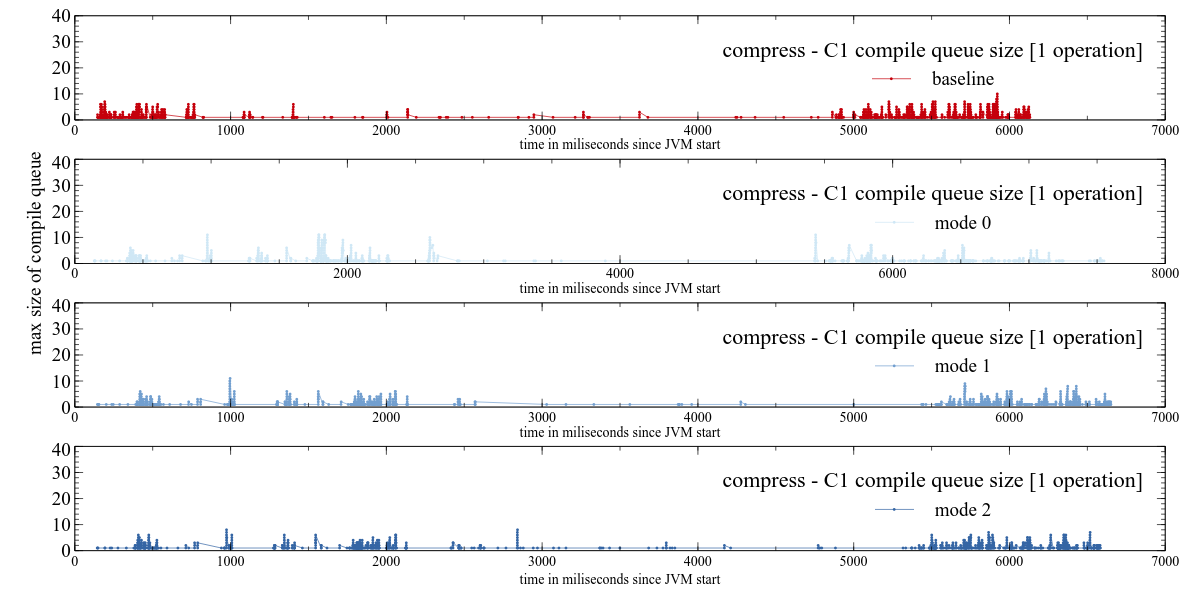
\includegraphics[width=1.0\textwidth]{figures/spec_queue_compress_separate_c1.png}
    \caption{C1 Compile queue size over time SPECjvm compress benchmark}
    \label{f:spec_queue_compress_separate_c1}
  \end{center}
\end{figure}
\begin{figure}[ht]
  \begin{center}
    \centering
    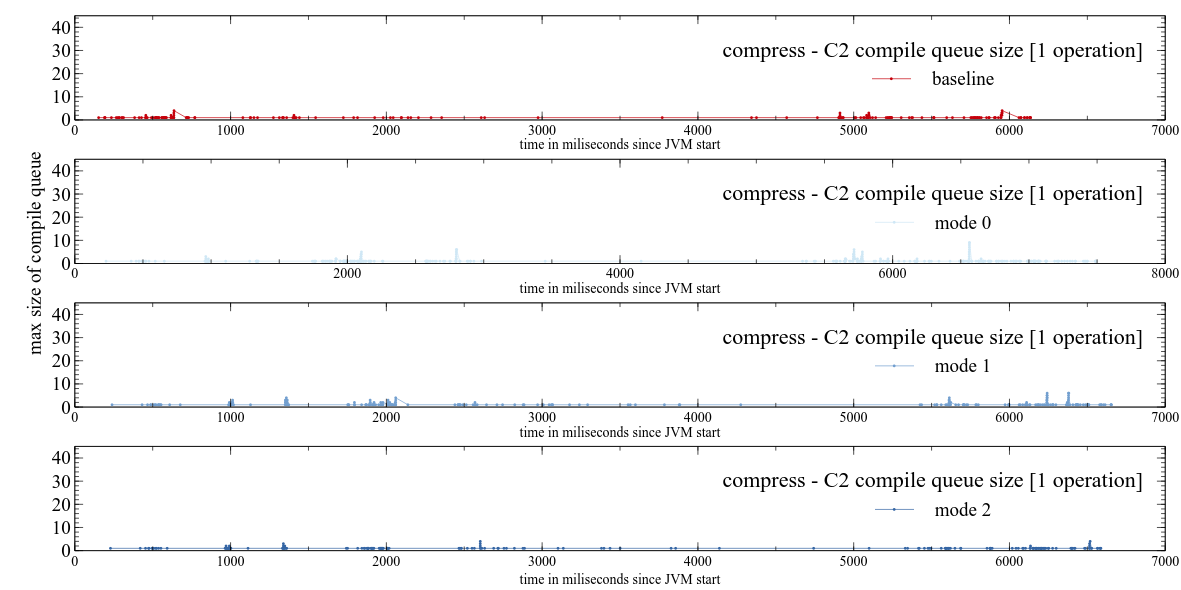
\includegraphics[width=1.0\textwidth]{figures/spec_queue_compress_separate_c2.png}
    \caption{C2 Compile queue size over time SPECjvm compress benchmark}
    \label{f:spec_queue_compress_separate_c2}
  \end{center}
\end{figure}
% --------------------------- SPECjvm scimark.sparse.large Queue ------------------
\begin{figure}[ht]
  \begin{center}
    \centering
    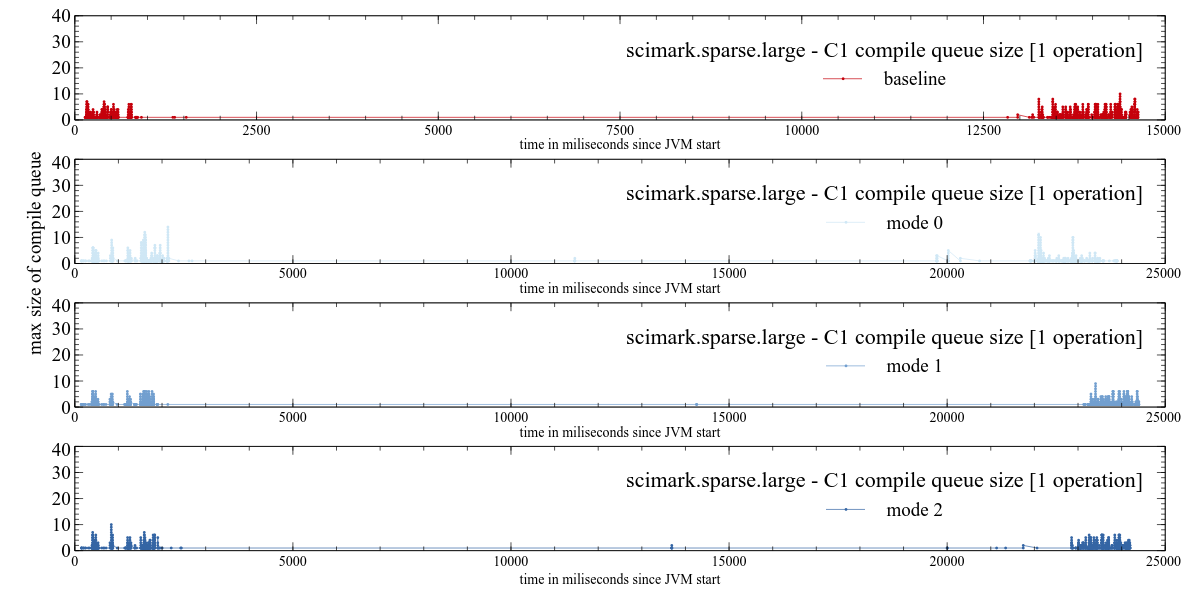
\includegraphics[width=1.0\textwidth]{figures/spec_queue_scirmarksparselarge_separate_c1.png}
    \caption{C1 Compile queue size over time SPECjvm scimark.sparse.large benchmark}
    \label{f:spec_queue_scirmarksparselarge_separate_c1}
  \end{center}
\end{figure}
\begin{figure}[ht]
  \begin{center}
    \centering
    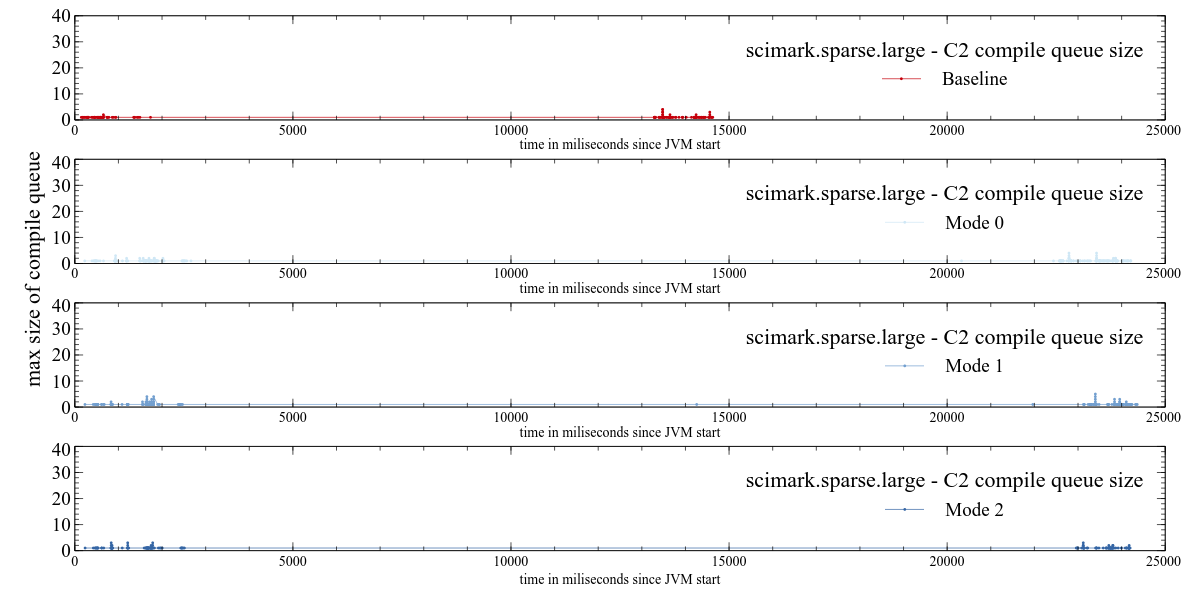
\includegraphics[width=1.0\textwidth]{figures/spec_queue_scirmarksparselarge_separate_c2.png}
    \caption{C2 Compile queue size over time SPECjvm scimark.sparse.large benchmark}
    \label{f:spec_queue_scirmarksparselarge_separate_c2}
  \end{center}
\end{figure}
